\chapter{Constantes de equilibrio y desplazamientos}\label{ch:b2:equilibrium-shifts}

Una planta de amoníaco hace funcionar su convertidor a unos \qty{450}{\celsius} y
\qty{200}{bar}. A temperatura ambiente el equilibrio \ce{N2 + 3H2 <=>
2NH3} está tan desplazado hacia el amoníaco que una mezcla de los elementos podría en
principio convertirse casi por completo; sin embargo, los ingenieros la calientan, lo que
hace retroceder el equilibrio, y luego la comprimen a doscientas
atmósferas, lo que cuesta mucha energía. Las razones son un
compromiso entre hasta dónde puede llegar una reacción y a qué velocidad lo hace. Este
capítulo convierte la \omterm{def:b2:reaction-free-energy:gibbs-energy}{energía de Gibbs} de los capítulos anteriores en la
constante de equilibrio del volumen del primer año, muestra cómo varía esa constante
con la temperatura, cuenta cuántas condiciones puede elegir libremente un
experimentador y predice en qué sentido se desplaza un equilibrio cuando se cambian la
temperatura, la presión o la composición.

\begin{recall}
\Cref{ch:b2:reaction-free-energy}: el criterio de evolución $\Delta_r G\,\dd\xi
\leq 0$ y la relación de Gibbs--Helmholtz;
\cref{ch:b2:chemical-potential}: $\Delta_r G = \Delta_r G^\circ + RT\ln Q$.
El volumen del primer año: el cociente $Q = \prod_i a_i^{\nu_i}$, la constante de
equilibrio estándar $K^\circ$ como valor de $Q$ en el equilibrio, la ley de
acción de masas y la regla ``$Q < K^\circ$: sentido directo'', todas enunciadas allí como
leyes; tablas de avance; estados finales de una o dos reacciones. También
prometía explicar aquí la elección de la temperatura y de la presión para el amoníaco y para
el trióxido de azufre.
\end{recall}

\begin{omfigure}
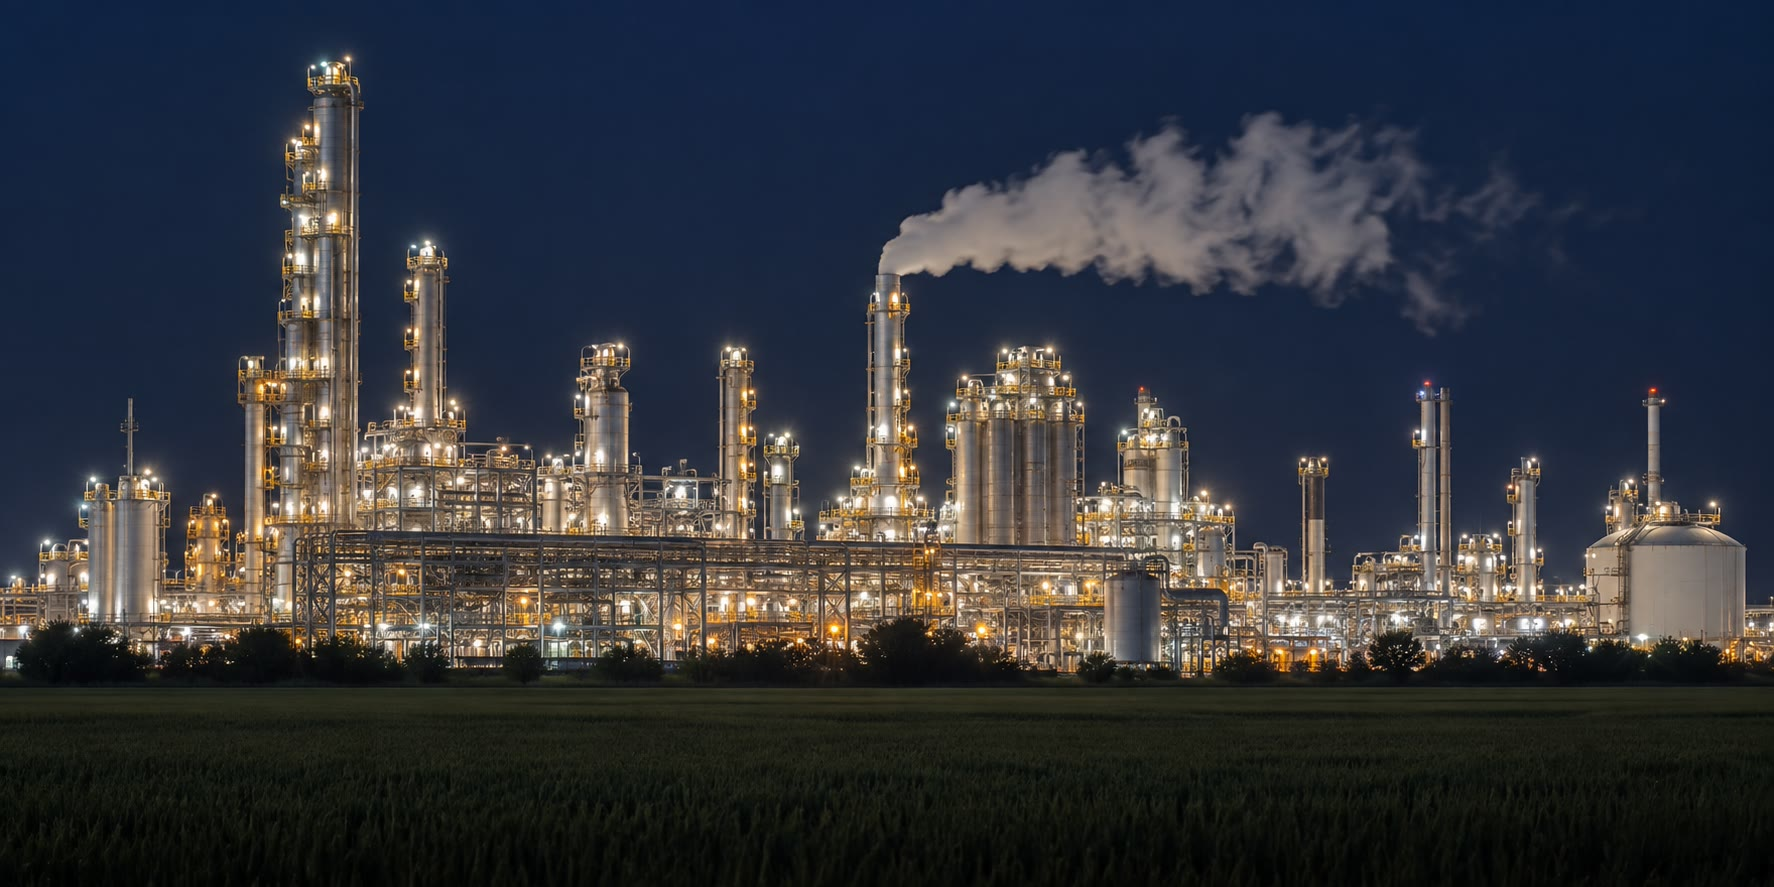
\includegraphics[width=0.7\linewidth]{images/book3/ai/b2-04-ammonia-plant.jpg}

{\small Una planta de amoníaco de noche. En su convertidor, el nitrógeno y el hidrógeno
pasan sobre un catalizador de hierro a unos cientos de grados y unos cientos de bar;
la elección de esas condiciones es el objeto del problema de fin de semana.}
\end{omfigure}

\section{La constante de equilibrio a partir de la energía de Gibbs}

\begin{theorem}[Constante de equilibrio estándar]\label{thm:b2:equilibrium-shifts:k-from-g}
En el equilibrio $\Delta_r G = 0$, y el cociente de reacción toma el valor
\[
  K^\circ(T) = \exp\!\left(-\frac{\Delta_r G^\circ(T)}{RT}\right), \qquad
  \Delta_r G^\circ(T) = -RT\ln K^\circ(T) .
\]
Solo depende de la temperatura.
\end{theorem}

\begin{proof}
El criterio de evolución hace de $\Delta_r G = 0$ la condición de equilibrio.
Con $\Delta_r G = \Delta_r G^\circ + RT\ln Q$
(\cref{prop:b2:chemical-potential:delta-g-q}), el equilibrio significa $\ln Q_{\text{eq}}
= -\Delta_r G^\circ/(RT)$, función solo de $T$ porque $\Delta_r G^\circ$ lo es.
\end{proof}

\begin{corollary}[Las leyes del volumen del primer año]\label{cor:b2:equilibrium-shifts:mass-action}
$\Delta_r G = RT\ln(Q/K^\circ)$. Por tanto, un sistema con $Q < K^\circ$ evoluciona
en sentido directo, uno con $Q > K^\circ$ en sentido inverso, y uno con $Q = K^\circ$ está en
equilibrio (la ley de acción de masas).
\end{corollary}

\begin{proof}
Se sustituye $\Delta_r G^\circ = -RT\ln K^\circ$ en $\Delta_r G = \Delta_r G^\circ
+ RT\ln Q$; el signo de $\Delta_r G$ es el de $\ln(Q/K^\circ)$, y el
criterio de evolución exige $\Delta_r G\,\dd\xi \leq 0$.
\end{proof}

\begin{example}[Tres constantes a \qty{298}{K}]\label{ex:b2:equilibrium-shifts:constants}
Síntesis del amoníaco, $\Delta_r G^\circ = \qty{-32.8}{kJ/mol}$: $K^\circ =
\exp(32\,800/(8.314 \times 298.15)) = \num{5.6e5}$ (las tablas, con más
cifras, dan \num{5.4e5}). La disociación de \ce{N2O4}, $\Delta_r G^\circ =
\qty{+4.7}{kJ/mol}$: $K^\circ = 0.15$. La descomposición de la caliza,
$\Delta_r G^\circ = \qty{+130.4}{kJ/mol}$: $K^\circ = \num{1.5e-23}$, y la
presión de equilibrio del dióxido de carbono sobre la caliza a temperatura ambiente
es de $\num{1.5e-23}$ bar, nada en absoluto. Una variación de \qty{5.7}{kJ/mol} en
$\Delta_r G^\circ$ a \qty{298}{K} multiplica o divide $K^\circ$ por diez.
% ledger: dfh:NH3_g, s0:NH3_g, janafG:NH3.298.15 (computed in figdata/bachelor-2/thermo-data.py and vant-hoff.py)
\end{example}

La \omterm{def:b2:reaction-free-energy:gibbs-energy}{energía de Gibbs} del sistema completo muestra lo mismo como un paisaje:
es mínima en el avance de equilibrio, donde su pendiente, $\Delta_r G$, es
nula.

\begin{omfigure}
\begin{tikzpicture}
\begin{axis}[
  width=0.7\linewidth, height=5.6cm, xmin=0, xmax=1, ymin=-2.2, ymax=5.2,
  axis x line=bottom, axis y line=left, xlabel={avance $\xi$ (mol)},
  ylabel={$G(\xi) - G(0)$ (\unit{kJ})},
  tick label style={font=\small}, label style={font=\small}, clip=false]
\addplot[omDef, very thick] table[x=xi, y=G] {figdata/out/bachelor-2-gibbs-extent.dat};
\draw[dotted] (axis cs:0.189,-2.2) -- (axis cs:0.189,-0.949);
\fill[omThm] (axis cs:0.189,-0.949) circle (1.6pt);
\node[omThm, anchor=west, font=\small] at (axis cs:0.21,-1.75) {equilibrio, $\xi = 0.189$};
\draw[dashed, gray] (axis cs:0,0) -- (axis cs:1,4.728);
\node[gray, font=\scriptsize, anchor=south east] at (axis cs:1,4.75) {$\xi\,\Delta_r G^\circ$};
\end{axis}
\end{tikzpicture}

{\small \omterm{def:b2:reaction-free-energy:gibbs-energy}{Energía de Gibbs} de un sistema cerrado de gases perfectos a \qty{298}{K} y
\qty{1}{bar}, partiendo de \qty{1}{mol} de \ce{N2O4}, en función del avance de
\ce{N2O4 <=> 2NO2}. Aunque $\Delta_r G^\circ > 0$ (recta discontinua, especies
puras), la mezcla de los dos gases rebaja $G$, y el mínimo está en $\xi =
0.189$, donde $Q = K^\circ = 0.15$. A su izquierda la pendiente $\Delta_r G =
\partial G/\partial\xi$ es negativa, a su derecha positiva.}
% ledger: dfh:N2O4_g, s0:N2O4_g, dfh:NO2_g, s0:NO2_g (computed in figdata/bachelor-2/gibbs-extent.py)
\end{omfigure}

\section{Temperatura: la ecuación de van 't Hoff}

\begin{theorem}[Ecuación de van 't Hoff]\label{thm:b2:equilibrium-shifts:vant-hoff}
\[
  \frac{\dd\ln K^\circ}{\dd T} = \frac{\Delta_r H^\circ(T)}{RT^2}
\]
(la \emph{ecuación de van 't Hoff}\index{ecuacion de van 't Hoff@ecuación de van 't Hoff}): la constante de
equilibrio de una reacción \omterm{def:b2:reaction-enthalpy:exothermic}{endotérmica} aumenta con la temperatura, y la de
una reacción \omterm{def:b2:reaction-enthalpy:exothermic}{exotérmica} disminuye.
\end{theorem}

\begin{proof}
Se escribe $\ln K^\circ = -\Delta_r G^\circ/(RT)$ y se usa la relación de
Gibbs--Helmholtz de la \cref{prop:b2:reaction-free-energy:gibbs-helmholtz},
\[
  \frac{\dd}{\dd T}\left(\frac{\Delta_r G^\circ}{T}\right) =
  -\frac{\Delta_r H^\circ}{T^2} ;
\]
se divide por $-R$.
\end{proof}

\begin{proposition}[Forma integrada]\label{prop:b2:equilibrium-shifts:integrated}
Si $\Delta_r H^\circ$ es constante entre $T_1$ y $T_2$ (\omterm{def:b2:reaction-free-energy:ellingham-approximation}{aproximación de
Ellingham}),
\[
  \ln\frac{K^\circ(T_2)}{K^\circ(T_1)} = -\frac{\Delta_r H^\circ}{R}\left(
  \frac{1}{T_2} - \frac{1}{T_1}\right),
\]
y $\ln K^\circ$ es una recta de pendiente $-\Delta_r H^\circ/R$ en función de
$1/T$.
\end{proposition}

\begin{proof}
Se integra $\dd\ln K^\circ = (\Delta_r H^\circ/R)\,\dd T/T^2$, observando que
$\dd T/T^2 = -\dd(1/T)$.
\end{proof}

\begin{omfigure}
\begin{tikzpicture}
\begin{axis}[
  width=0.72\linewidth, height=5.8cm, xmin=0.9, xmax=3.5, ymin=-19, ymax=15,
  axis x line=bottom, axis y line=left, xlabel={$1000/T$ (\unit{1/K})},
  ylabel={$\ln K^\circ$}, tick label style={font=\small},
  label style={font=\small}, clip=false]
\addplot[omThm, dashed, thick] table[x=invT, y=lnK] {figdata/out/bachelor-2-vant-hoff-a-line.dat};
\addplot[omDef, only marks, mark=*, mark size=1.8pt] table[x=invT, y=lnK] {figdata/out/bachelor-2-vant-hoff-a.dat};
\node[omDef, font=\scriptsize, anchor=west] at (axis cs:3.36,13.2) {\qty{298}{K}};
\node[omDef, font=\scriptsize, anchor=north west] at (axis cs:1.03,-15.3) {\qty{1000}{K}};
\node[omThm, font=\small, anchor=south east, align=right] at (axis cs:2.4,8) {pendiente $-\Delta_r H^\circ(298)/R$\\ $= +11\,050$ K};
\end{axis}
\end{tikzpicture}

{\small La constante de \ce{N2 + 3H2 <=> 2NH3} según las tablas (puntos, de 298 a
\qty{1000}{K}) y la recta de van 't Hoff trazada con $\Delta_r H^\circ$ a
\qty{298}{K} (discontinua). La reacción es \omterm{def:b2:reaction-enthalpy:exothermic}{exotérmica}: $K^\circ$ cae de
\num{5e5} a \num{3e-7}. A alta temperatura los puntos quedan por debajo de la recta:
$\Delta_r H^\circ$ se vuelve más negativa a medida que $T$ aumenta
(\cref{ex:b2:reaction-enthalpy:kirchhoff}).}
% ledger: janafG:NH3.298.15, janafG:NH3.400, janafG:NH3.500, janafG:NH3.600, janafG:NH3.700, janafG:NH3.800, janafG:NH3.900, janafG:NH3.1000, dfh:NH3_g (computed in figdata/bachelor-2/vant-hoff.py)
\end{omfigure}

\begin{method}[Una constante de equilibrio a otra temperatura]\label{met:b2:equilibrium-shifts:k-at-t}
\begin{enumerate}
  \item Con las tablas a \qty{298}{K}, calcúlense $\Delta_r H^\circ$, $\Delta_r
        S^\circ$ y $K^\circ(298)$.
  \item O bien se usa la \omterm{thm:b2:equilibrium-shifts:vant-hoff}{ecuación de van 't Hoff} integrada, o bien se calcula
        $\Delta_r G^\circ(T) = \Delta_r H^\circ - T\Delta_r S^\circ$ y luego
        $K^\circ(T)$: ambas son la misma aproximación.
  \item Para un intervalo amplio o una $\Delta_r C_p^\circ$ grande, son preferibles los valores tabulados
        de $\Delta_f G^\circ(T)$; un error de \qty{5.7}{kJ/mol} a \qty{298}{K}
        (o de \qty{13}{kJ/mol} a \qty{700}{K}) es un factor diez en $K^\circ$.
\end{enumerate}
\end{method}

\begin{history}[Jacobus Henricus van 't Hoff]
\begin{minipage}[t]{0.2\linewidth}\vspace{0pt}
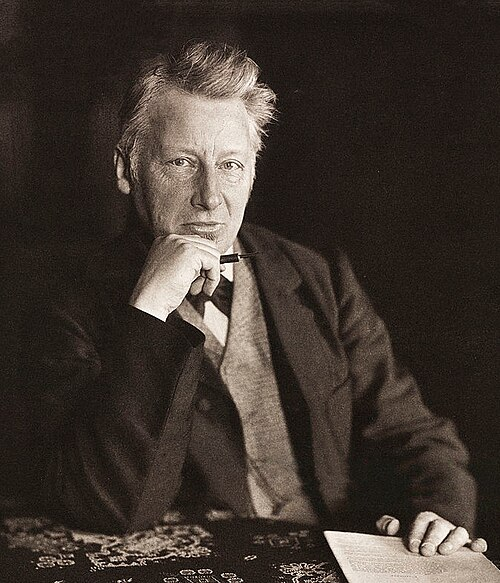
\includegraphics[width=\linewidth]{images/book3/vanthoff.jpg}
\end{minipage}\hfill
\begin{minipage}[t]{0.76\linewidth}\vspace{0pt}
Jacobus Henricus van 't Hoff (1852--1911) dio en 1884, en sus
\emph{Études de dynamique chimique}, la relación entre la temperatura y
la constante de equilibrio que lleva su nombre, y al año siguiente la ley de la
\omterm{def:b2:chemical-potential:osmotic-pressure}{presión osmótica} del \cref{ch:b2:chemical-potential}; diez años antes había
propuesto el átomo de carbono tetraédrico. Recibió el primer Premio Nobel de
Química, en 1901. (Fotografía de N. Perscheid, 1904: dominio público,
Wikimedia Commons.)
\end{minipage}
\end{history}

\section{Varianza}

¿Cuántas magnitudes intensivas puede fijar libremente un experimentador antes de que el
estado de equilibrio quede completamente determinado?

\begin{definition}[Varianza]\label{def:b2:equilibrium-shifts:variance}
Los \emph{parámetros intensivos independientes}\index{parametro intensivo independiente@parámetro intensivo independiente}
de un sistema en equilibrio son un conjunto de magnitudes intensivas
(temperatura, presión, fracciones molares en cada fase) que pueden elegirse
independientemente y que, una vez elegidas, fijan todas las demás. Su número es la
\emph{varianza}\index{varianza} $v$ del sistema.
\end{definition}

\begin{theorem}[Regla de las fases]\label{thm:b2:equilibrium-shifts:phase-rule}
Para un sistema de $n$ especies repartidas entre $\varphi$ fases, ligadas por $r$
reacciones de equilibrio independientes y por $s$ relaciones adicionales entre
magnitudes intensivas fijadas por la preparación (una alimentación estequiométrica,
la electroneutralidad),
\[
  v = c + 2 - \varphi, \qquad c = n - r - s .
\]
\end{theorem}

\begin{proof}
Variables intensivas: $T$, $p$ y, en cada fase, las fracciones molares de las
$n$ especies, que suman 1, es decir, $n - 1$ libres por fase: en total $2 +
\varphi(n - 1)$. Relaciones: cada especie está en equilibrio entre las
fases, $\varphi - 1$ igualdades de \omterm{def:b2:chemical-potential:chemical-potential}{potenciales químicos} por especie, $n(\varphi -
1)$ en total; cada reacción da $Q = K^\circ(T)$, $r$ relaciones; y $s$
relaciones adicionales. Restando: $v = 2 + \varphi(n - 1) - n(\varphi - 1) - r -
s = n - r - s + 2 - \varphi$. (Una especie ausente de una fase elimina a la vez una
variable y una relación.)
\end{proof}

\begin{method}[Cálculo de una varianza]\label{met:b2:equilibrium-shifts:variance}
\begin{enumerate}
  \item Enumérense las especies, con su fase, y cuéntense $n$ y $\varphi$
        (cada sólido puro es una fase; todos los gases forman una sola fase).
  \item Cuéntense las reacciones independientes $r$ entre ellas.
  \item Cuéntense las relaciones adicionales $s$: cantidades en proporción estequiométrica
        (solo si la relación liga magnitudes de una misma fase),
        electroneutralidad de una disolución iónica.
  \item $v = n - r - s + 2 - \varphi$.
\end{enumerate}
\end{method}

\begin{example}[Tres varianzas]\label{ex:b2:equilibrium-shifts:variances}
Caliza en un recipiente cerrado, \ce{CaCO3(s) <=> CaO(s) + CO2(g)}: $n = 3$, $r =
1$, $\varphi = 3$ (dos sólidos y un gas): $v = 1$. Se elige $T$, y la presión
del dióxido de carbono queda fijada: $p = K^\circ(T)\,p^\circ$. Una mezcla gaseosa de
\ce{N2}, \ce{H2} y \ce{NH3} en equilibrio: $n = 3$, $r = 1$, $\varphi = 1$, $v
= 3$ ($T$, $p$ y una variable de composición); preparada a partir de amoníaco solo, o de
una alimentación estequiométrica, \ce{N2} y \ce{H2} están en la proporción 1 : 3, $s = 1$ y
$v = 2$: a $T$ y $p$ dadas la composición queda fijada, como aprovecha el problema de fin
de semana.
\end{example}

\section{Desplazamiento de un equilibrio}

\begin{definition}[Desplazamiento de un equilibrio]\label{def:b2:equilibrium-shifts:shift}
Cuando un sistema en equilibrio se perturba (un cambio de temperatura, de
presión o de una cantidad), en general deja de estar en equilibrio y
evoluciona hacia uno nuevo. El \emph{desplazamiento del equilibrio}\index{desplazamiento de un equilibrio}
es en sentido directo si la reacción avanza ($\dd\xi > 0$) y en sentido inverso
en caso contrario.
\end{definition}

\begin{method}[Predecir un desplazamiento]\label{met:b2:equilibrium-shifts:predict-shift}
Justo después de la perturbación, calcúlense $Q$ y $K^\circ$ (o estímese el signo de su
variación). Si ahora $Q < K^\circ$, el desplazamiento es en sentido directo; si $Q > K^\circ$,
en sentido inverso; si la igualdad se mantiene, no hay desplazamiento.
\end{method}

\begin{omfigure}
\begin{tikzpicture}[font=\small, >={Stealth}]
  \draw[->, thick] (0,0) -- (11,0) node[right] {$\ln Q$};
  \draw[omThm, thick] (5.5,0.25) -- (5.5,-0.25) node[below, align=center] {$\ln K^\circ$\\ ($= \ln Q$ antes)};
  \fill (5.5,0) circle (2pt);
  \draw[omDef, thick] (2.8,0.25) -- (2.8,-0.25) node[below] {$\ln Q$ justo después};
  \draw[->, omDef, very thick] (3.0,0.6) -- (5.2,0.6) node[midway, above] {sentido directo};
  \draw[omProp, thick] (8.4,0.25) -- (8.4,-0.25) node[below] {$\ln Q$ justo después};
  \draw[->, omProp, very thick] (8.2,0.6) -- (5.8,0.6) node[midway, above] {sentido inverso};
\end{tikzpicture}

{\small Una perturbación desplaza $Q$ (o $K^\circ$, si cambia la temperatura);
el sistema evoluciona entonces hasta que vuelve a cumplirse $Q = K^\circ$, en sentido directo si $Q$ se ha vuelto
demasiado pequeño, en sentido inverso si es demasiado grande.}
\end{omfigure}

\begin{proposition}[Temperatura]\label{prop:b2:equilibrium-shifts:temperature}
A presión constante, elevar la temperatura desplaza un equilibrio en el
sentido \omterm{def:b2:reaction-enthalpy:exothermic}{endotérmico} (directo si $\Delta_r H^\circ > 0$), y bajarla, en el
sentido \omterm{def:b2:reaction-enthalpy:exothermic}{exotérmico}.
\end{proposition}

\begin{proof}
A composición y presión fijas, $Q$ no varía con $T$ (para sistemas
ideales); por van 't Hoff, $K^\circ$ aumenta con $T$ si $\Delta_r H^\circ >
0$. Justo después de una subida de $T$, por tanto, $Q < K^\circ$: sentido directo.
\end{proof}

\begin{proposition}[Presión]\label{prop:b2:equilibrium-shifts:pressure}
A temperatura y composición constantes, elevar la presión total de un
equilibrio en fase gaseosa lo desplaza en el sentido que reduce el número de
moléculas de gas (sentido directo si $\Delta\nu_{\text{gas}} < 0$). Si $\Delta\nu_{\text{gas}}
= 0$, la presión no tiene efecto.
\end{proposition}

\begin{proof}
Con $p_i = x_ip$, $Q = \prod_i x_i^{\nu_i}\,(p/p^\circ)^{\Delta\nu_{\text{gas}}}$:
a composición fija, elevar $p$ multiplica $Q$ por
$(p'/p)^{\Delta\nu_{\text{gas}}}$, que es $< 1$ si $\Delta\nu_{\text{gas}} <
0$. Entonces $Q < K^\circ$: sentido directo. Las fases condensadas no contribuyen.
\end{proof}

\begin{proposition}[Adición de un constituyente o de un gas inerte]\label{prop:b2:equilibrium-shifts:adding}
Añadir una pequeña cantidad de un constituyente gaseoso $j$ a un equilibrio en fase gaseosa
hace variar $\ln Q$ en
\[
  \left(\frac{\partial\ln Q}{\partial n_j}\right) = \frac{\nu_j}{n_j} -
  \frac{\Delta\nu_{\text{gas}}}{n_{\text{tot}}}\ \ \text{fijando } T, p ;
  \qquad \frac{\nu_j}{n_j}\ \ \text{fijando } T, V .
\]
Añadir un gas inerte no tiene efecto a volumen constante, y a presión constante
actúa como una disminución de la presión.
\end{proposition}

\begin{proof}
A $T$, $p$ constantes: $Q = \prod_i n_i^{\nu_i}\,(p/(p^\circ n_{\text{tot}}))^{
\Delta\nu_{\text{gas}}}$, cuya derivada logarítmica respecto de $n_j$ es
$\nu_j/n_j - \Delta\nu_{\text{gas}}/n_{\text{tot}}$ (primer término nulo para un gas
inerte, $\nu_j = 0$). A $T$, $V$ constantes: $p_i = n_iRT/V$ y $Q = \prod_i n_i^{
\nu_i}\,(RT/(p^\circ V))^{\Delta\nu_{\text{gas}}}$, cuya derivada es
solo $\nu_j/n_j$.
\end{proof}

\begin{remark}[Un reactivo añadido que hace retroceder la reacción]\label{rem:b2:equilibrium-shifts:paradox}
En la síntesis del amoníaco, $\nu(\ce{N2}) = -1$ y $\Delta\nu_{\text{gas}} = -2$:
añadir nitrógeno a $T$ y $p$ constantes hace variar $\ln Q$ en $-1/n_{\ce{N2}} +
2/n_{\text{tot}}$, que es positivo cuando $x(\ce{N2}) > 1/2$. En una mezcla
ya rica en nitrógeno, añadir más nitrógeno diluye tanto el hidrógeno
que el amoníaco se descompone. La regla ``añadir un reactivo desplaza en sentido directo'' es segura
a volumen constante, no siempre a presión constante.
\end{remark}

\begin{proposition}[Principio de Le Chatelier]\label{prop:b2:equilibrium-shifts:le-chatelier}
Las proposiciones anteriores se resumen en el \emph{principio de Le
Chatelier}\index{principio de Le Chatelier}: un sistema en equilibrio,
perturbado en temperatura o en presión, se desplaza en el sentido que se opone a
la perturbación (absorbe calor cuando se calienta, reduce su volumen gaseoso cuando se
comprime).
\end{proposition}

\begin{proof}
Reformula la \cref{prop:b2:equilibrium-shifts:temperature} (el sentido
\omterm{def:b2:reaction-enthalpy:exothermic}{endotérmico} absorbe calor) y la \cref{prop:b2:equilibrium-shifts:pressure} (menos
moléculas de gas ocupan menos volumen a las mismas $T$ y $p$). Para adiciones de
materia a presión constante el principio no es fiable
(\cref{rem:b2:equilibrium-shifts:paradox}): calcúlese $Q$.
\end{proof}

\begin{remark}[Cuando el equilibrio se rompe]\label{rem:b2:equilibrium-shifts:rupture}
Un desplazamiento puede terminar no en un nuevo equilibrio sino en la desaparición de una fase.
Calentada en un recipiente cerrado, la caliza se descompone hasta que $p(\ce{CO2}) =
K^\circ(T)\,p^\circ$; si no hay suficiente para alcanzar esa presión,
desaparece por completo y $Q$ queda por debajo de $K^\circ$: el sistema queda fuera de
equilibrio definitivamente, como ya observó el volumen del primer año.
\end{remark}

\begin{history}[Henry Le Chatelier]
\begin{minipage}[t]{0.2\linewidth}\vspace{0pt}
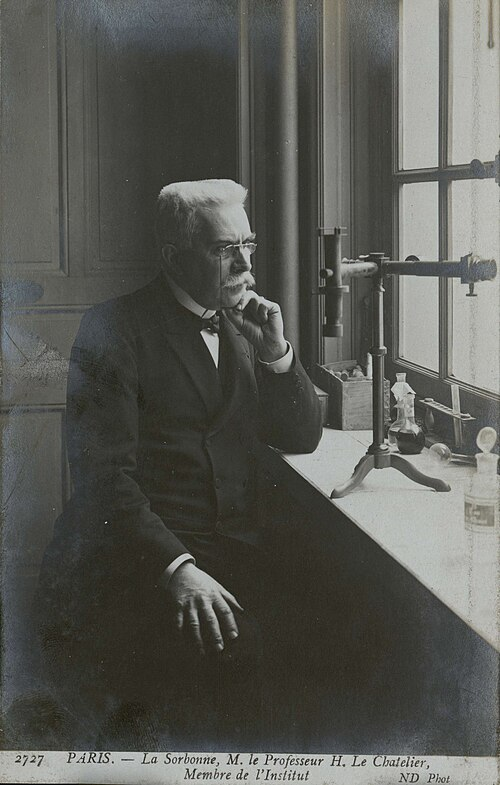
\includegraphics[width=\linewidth]{images/book3/lechatelier.jpg}
\end{minipage}\hfill
\begin{minipage}[t]{0.76\linewidth}\vspace{0pt}
Henry Le Chatelier (1850--1936), ingeniero de minas y químico que trabajó en
cementos, metalurgia y pirometría, enunció en 1884 la ``ley de \omterm{def:b2:equilibrium-shifts:shift}{desplazamiento
del equilibrio}'' que lleva su nombre. Hacia 1901 también intentó obtener
amoníaco a partir de sus elementos a presión; una explosión en su aparato puso fin
al intento. (Fotografía: autor desconocido, CC BY-SA 4.0, Wikimedia Commons.)
\end{minipage}
\end{history}

\section{Optimizar una síntesis}

\subsection*{El amoníaco}

\begin{omfigure}
\begin{tikzpicture}
\begin{axis}[
  width=0.78\linewidth, height=6.2cm, xmin=500, xmax=1000, ymin=0, ymax=0.9,
  axis x line=bottom, axis y line=left, xlabel={$T$ (K)},
  ylabel={fracción molar de \ce{NH3} en el equilibrio},
  tick label style={font=\small}, label style={font=\small}, clip=false]
\addplot[omThm, very thick] table[x=T, y=p300] {figdata/out/bachelor-2-vant-hoff-b.dat};
\addplot[omDef, very thick] table[x=T, y=p200] {figdata/out/bachelor-2-vant-hoff-b.dat};
\addplot[omProp, very thick] table[x=T, y=p50] {figdata/out/bachelor-2-vant-hoff-b.dat};
\addplot[black!60, very thick] table[x=T, y=p1] {figdata/out/bachelor-2-vant-hoff-b.dat};
\node[omThm, font=\scriptsize, anchor=south west] at (axis cs:600,0.70) {300 bar};
\node[omDef, font=\scriptsize, anchor=north east] at (axis cs:612,0.52) {200 bar};
\node[omProp, font=\scriptsize, anchor=north east] at (axis cs:578,0.30) {50 bar};
\node[black!60, font=\scriptsize, anchor=south west] (onebar) at (axis cs:520,0.13) {1 bar};
\draw[black!60] (onebar.south west) -- (axis cs:512,0.075);
\draw[dotted] (axis cs:723,0) -- (axis cs:723,0.253);
\fill[omDef] (axis cs:723,0.253) circle (1.6pt);
\end{axis}
\end{tikzpicture}

{\small Fracción molar de amoníaco en el equilibrio a partir de una mezcla 1 : 3 de nitrógeno
e hidrógeno (gases perfectos), en función de la temperatura a cuatro presiones,
calculada a partir de las \omterm{def:b2:reaction-free-energy:gibbs-energy}{energías de Gibbs} tabuladas. La presión la aumenta, la temperatura
la disminuye; el punto marca \qty{723}{K} y \qty{200}{bar}.}
% ledger: janafG:NH3.500, janafG:NH3.600, janafG:NH3.700, janafG:NH3.800, janafG:NH3.900, janafG:NH3.1000 (computed in figdata/bachelor-2/vant-hoff.py)
\end{omfigure}

La síntesis es \omterm{def:b2:reaction-enthalpy:exothermic}{exotérmica} y reduce cuatro moléculas de gas a dos: según
las proposiciones anteriores, la temperatura baja y la presión alta favorecen el amoníaco.
A \qty{1}{bar} y a temperatura ambiente el equilibrio es casi completo, pero
la reacción no tiene lugar en absoluto: el triple enlace del nitrógeno solo se rompe
sobre un catalizador, y el catalizador de hierro solo funciona a varios cientos de
grados. Las plantas eligen, por tanto:
\begin{itemize}
  \item una temperatura suficientemente alta para la velocidad, tan baja como permita el catalizador
        (en torno a \qty{700}{K});
  \item una presión alta para recuperar el rendimiento perdido por la temperatura, limitada
        por el coste de la compresión y de los recipientes de paredes gruesas;
  \item un bucle: el gas que sale del convertidor se enfría, el amoníaco se condensa
        y se retira, y el gas no convertido se recicla con alimentación fresca;
        una pequeña \omterm{def:b2:equilibrium-shifts:single-pass}{purga} elimina el argón y el metano que, si no, se
        acumularían.
\end{itemize}

\begin{definition}[Conversión por paso, reciclado, purga]\label{def:b2:equilibrium-shifts:single-pass}
En un proceso con reciclado, la \emph{conversión por paso}\index{conversion por paso@conversión por paso}
es la fracción de un reactivo convertida en un solo paso por
el reactor; la parte no convertida, separada del producto, se devuelve
a la entrada del reactor como \emph{reciclado}\index{reciclado}; una
\emph{purga}\index{purga} es una pequeña corriente extraída continuamente del
reciclado para evitar que se acumulen las especies inertes.
\end{definition}

\begin{omfigure}
\begin{tikzpicture}[font=\small, >={Stealth}, box/.style={draw, thick, rounded corners=2pt, minimum width=2.1cm, minimum height=1.0cm, align=center, fill=white}]
  \node[box] (comp) at (0,0) {compresor};
  \node[box] (conv) at (3.6,0) {convertidor\\ (catalizador)};
  \node[box] (cond) at (7.2,0) {enfriador y\\ separador};
  \draw[->, thick] (-3.9,0) -- (comp) node[pos=0.0, above right] {\ce{N2 + 3H2} fresco};
  \draw[->, thick] (comp) -- (conv);
  \draw[->, thick] (conv) -- (cond);
  \draw[->, thick, omDef] (cond.south) -- ++(0,-1.0) node[below] {amoníaco líquido};
  \draw[->, thick, omThm] (cond.north) -- ++(0,0.9) -| (comp.north);
  \node[omThm, above] at (2.6,1.4) {reciclado (gas no convertido)};
  \draw[->, thick, black!60] (6.1,1.4) -- (6.1,2.1) node[above] {purga};
\end{tikzpicture}

{\small El bucle del amoníaco. Cada paso solo convierte una parte del gas; el amoníaco
se separa por condensación, y el resto se recomprime y se devuelve con la alimentación
fresca. La \omterm{def:b2:equilibrium-shifts:single-pass}{purga} impide que se acumulen el argón y el metano, que no
reaccionan.}
\end{omfigure}

\begin{history}[Haber and Bosch]
\begin{minipage}[t]{0.15\linewidth}\vspace{0pt}
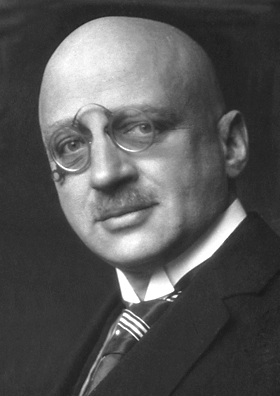
\includegraphics[width=\linewidth]{images/book3/haber.png}
\end{minipage}\hspace{0.01\linewidth}%
\begin{minipage}[t]{0.15\linewidth}\vspace{0pt}
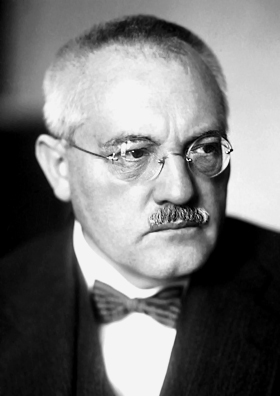
\includegraphics[width=\linewidth]{images/book3/bosch.jpg}
\end{minipage}\hfill
\begin{minipage}[t]{0.66\linewidth}\vspace{0pt}
Fritz Haber (1868--1934) midió el equilibrio del amoníaco a presión
y, en 1909, lo hizo salir de forma continua de un convertidor de laboratorio sobre un
catalizador de osmio. Carl Bosch (1874--1940) lo convirtió en una industria, con
recipientes de acero que resistían el hidrógeno caliente a presión y un catalizador
barato de hierro; la primera planta arrancó en 1913. Haber recibió el Premio Nobel en
1918, y Bosch en 1931. (Retratos de la Fundación Nobel: dominio público, Wikimedia
Commons.)
\end{minipage}
\end{history}

\subsection*{El trióxido de azufre}

En el proceso de contacto, \ce{2SO2(g) + O2(g) <=> 2SO3(g)} ($\Delta_r H^\circ =
\qty{-197.8}{kJ/mol}$ para la ecuación tal como está escrita) transcurre sobre un catalizador de
óxido de vanadio, activo solo en caliente, en varios lechos adiabáticos. En cada lecho el
calor liberado eleva la temperatura, lo que disminuye $K^\circ$; la conversión
se detiene cuando el gas alcanza la curva de equilibrio. Enfriar entre lechos lo
devuelve a una temperatura en la que el equilibrio permite más conversión.
% ledger: dfh:SO2_g, dfh:SO3_g

\begin{omfigure}
\begin{tikzpicture}
\begin{axis}[
  width=0.72\linewidth, height=6.4cm, xmin=600, xmax=900, ymin=0, ymax=1.08,
  axis x line=bottom, axis y line=left, xlabel={$T$ (K)},
  ylabel={conversión de \ce{SO2}}, tick label style={font=\small},
  label style={font=\small}, clip=false]
\addplot[black, very thick] table[x=T, y=X] {figdata/out/bachelor-2-vant-hoff-c.dat};
\addplot[omThm, thick] table[x=T, y=X] {figdata/out/bachelor-2-vant-hoff-bed1.dat};
\addplot[omThm, thick] table[x=T, y=X] {figdata/out/bachelor-2-vant-hoff-bed2.dat};
\addplot[omThm, thick] table[x=T, y=X] {figdata/out/bachelor-2-vant-hoff-bed3.dat};
\draw[->, omDef, thick] (axis cs:892.8,0.676) -- (axis cs:712,0.676);
\draw[->, omDef, thick] (axis cs:784.4,0.924) -- (axis cs:712,0.924);
\node[font=\scriptsize, anchor=south west] at (axis cs:860,0.84) {equilibrio};
\node[omThm, font=\scriptsize, anchor=west] at (axis cs:800,0.24) {lecho 1 (adiabático)};
\node[omDef, font=\scriptsize, anchor=south] at (axis cs:800,0.68) {enfriamiento};
\end{axis}
\end{tikzpicture}

{\small Conversión de equilibrio de \ce{SO2} en \ce{SO3} en función de la temperatura
(negro) para una alimentación modelo con un \qty{10}{\percent} de \ce{SO2} y un \qty{11}{\percent} de
\ce{O2} a \qty{1}{bar}, y trayectoria del gas a través de tres lechos adiabáticos
(rojo, con temperatura creciente porque la reacción calienta el gas), enfriado entre
lechos (azul).}
% ledger: janafG:SO2.600, janafG:SO2.700, janafG:SO2.800, janafG:SO2.900, janafG:SO3.600, janafG:SO3.700, janafG:SO3.800, janafG:SO3.900 (computed in figdata/bachelor-2/vant-hoff.py; feed and adiabatic rise are model values)
\end{omfigure}

\section{Ejercicios}

\begin{exercise}[$\star$]\label{exo:b2:equilibrium-shifts:1}
Calcúlese $K^\circ$ a \qty{298}{K} para una reacción con $\Delta_r G^\circ =
\qty{-32.8}{kJ/mol}$, y después para $\Delta_r G^\circ = \qty{+32.8}{kJ/mol}$.
¿Qué variación de $\Delta_r G^\circ$ multiplica $K^\circ$ por 100?
\end{exercise}

\begin{exercise}[$\star$]\label{exo:b2:equilibrium-shifts:2}
Para la síntesis del amoníaco, $K^\circ(298) = \num{5.4e5}$ y $\Delta_r H^\circ =
\qty{-91.9}{kJ/mol}$. Estímese $K^\circ$ a \qty{400}{K} con la \omterm{thm:b2:equilibrium-shifts:vant-hoff}{ecuación de
van 't Hoff} integrada; las tablas dan 35.6.
\end{exercise}

\begin{exercise}[$\star$]\label{exo:b2:equilibrium-shifts:3}
Calcúlese la \omterm{def:b2:equilibrium-shifts:variance}{varianza} de: (a) agua líquida en equilibrio con su vapor;
(b) \ce{CaCO3(s) <=> CaO(s) + CO2(g)} en un recipiente cerrado; (c) \ce{N2},
\ce{H2} y \ce{NH3} en equilibrio, con alimentación arbitraria; (d) \ce{C(s) + H2O(g) <=>
CO(g) + H2(g)}.
\end{exercise}

\begin{exercise}[$\star$]\label{exo:b2:equilibrium-shifts:4}
Para \ce{N2O4(g) <=> 2NO2(g)}, $\Delta_r H^\circ > 0$. ¿En qué sentido se desplaza el
equilibrio al calentar a presión constante, al comprimir a
temperatura constante y al añadir argón a volumen constante?
\end{exercise}

\begin{exercise}[$\star\star$]\label{exo:b2:equilibrium-shifts:5}
Para \ce{N2(g) + O2(g) <=> 2NO(g)}, $\Delta_r H^\circ = \qty{180.6}{kJ/mol}$ y
$\Delta_r S^\circ = \qty{24.8}{J/(K.mol)}$. Calcúlense $K^\circ$ a \qty{298}{K}
y a \qty{2000}{K} (\omterm{def:b2:reaction-free-energy:ellingham-approximation}{aproximación de Ellingham}), y la fracción molar de
\ce{NO} en el aire ($x(\ce{N2}) = 0.78$, $x(\ce{O2}) = 0.21$, poco consumidos) en el
equilibrio a \qty{2000}{K}. ¿Por qué producen los motores este contaminante, y por qué
sobrevive en los gases de escape enfriados?
\end{exercise}

\begin{exercise}[$\star\star$]\label{exo:b2:equilibrium-shifts:6}
Una esterificación $\mathrm{A + B \rightleftharpoons E + W}$ en fase líquida
tiene $K^\circ = 4.0$ (actividades tomadas como fracciones molares). Partiendo de
\qty{1.0}{mol} de ácido A, calcúlese la cantidad de éster con \qty{1.0}{mol} y luego
con \qty{3.0}{mol} de alcohol B. Explíquese, con $Q$ y $K^\circ$, por qué eliminar el
agua a medida que se forma lleva la reacción hasta el final.
\end{exercise}

\begin{exercise}[$\star\star$]\label{exo:b2:equilibrium-shifts:7}
A \qty{298}{K} y \qty{1}{bar}, $K^\circ = 0.148$ para \ce{N2O4 <=> 2NO2}.
Calcúlese el coeficiente de disociación de \qty{1}{mol} de \ce{N2O4}. Se añade después
\qty{1}{mol} de argón a presión total constante: calcúlese el nuevo
coeficiente de disociación, y explíquese. ¿Qué ocurre si el argón se añade a
volumen constante?
\end{exercise}

\begin{exercise}[$\star\star$]\label{exo:b2:equilibrium-shifts:8}
El cloruro de amonio sublima disociándose, \ce{NH4Cl(s) <=> NH3(g) +
HCl(g)}. Calcúlese la \omterm{def:b2:equilibrium-shifts:variance}{varianza} cuando el gas procede solo del sólido, y cuando
se ha añadido algo de amoníaco. ¿Qué significa cada caso para el experimentador?
\end{exercise}

\begin{exercise}[$\star\star$]\label{exo:b2:equilibrium-shifts:9}
Las tablas dan, para la síntesis del amoníaco, $K^\circ = 0.0993$ a \qty{500}{K} y
$K^\circ = \num{1.72e-3}$ a \qty{600}{K}. Dedúzcase $\Delta_r H^\circ$ en ese
intervalo y compárese con su valor a \qty{298}{K}.
\end{exercise}

\begin{exercise}[$\star\star\star$]\label{exo:b2:equilibrium-shifts:10}
Demuéstrese el contraejemplo de la \cref{rem:b2:equilibrium-shifts:paradox}: escríbase
$Q$ de la síntesis del amoníaco con las cantidades y la presión total, calcúlese
$\partial\ln Q/\partial n(\ce{N2})$ a $T$ y $p$ constantes, y hállese la
condición sobre $x(\ce{N2})$ para la cual añadir nitrógeno desplaza el equilibrio
en sentido inverso. ¿Puede ocurrir lo mismo a volumen constante?
\end{exercise}

\begin{exercise}[$\star\star\star$]\label{exo:b2:equilibrium-shifts:11}
Se calienta caliza a \qty{1100}{K} en un recipiente cerrado, inicialmente vacío, de
\qty{10.0}{L}, donde $\Delta_r G^\circ = \qty{1.62}{kJ/mol}$ para su
descomposición (\cref{ch:b2:reaction-free-energy}). Calcúlense $K^\circ$ y la
presión de equilibrio del dióxido de carbono. Hállese el estado final para
\qty{0.050}{mol} y para \qty{0.200}{mol} de caliza.
\end{exercise}

\begin{exercise}[$\star\star\star$]\label{exo:b2:equilibrium-shifts:12}
Léanse en la figura del proceso de contacto la conversión y la temperatura a la
salida de cada lecho. Explíquese por qué un solo lecho adiabático, por largo que fuera, no
podría superar en torno a un 68\,\% de conversión con esta alimentación, por qué el gas se enfría
entre lechos en lugar de mantener frío el catalizador todo el tiempo, y qué limita
la conversión del último lecho.
\end{exercise}

\section{Problema: el bucle del amoníaco}

\begin{problem}[{Problema de fin de semana --- la constante de equilibrio de la síntesis
del amoníaco y su dependencia de la temperatura, la composición en las condiciones
del convertidor, los desplazamientos debidos a la presión, la temperatura y los gases inertes, y
el bucle}]
\label{pb:b2:equilibrium-shifts:1}
El amoníaco se obtiene por \ce{N2(g) + 3H2(g) <=> 2NH3(g)} a partir de una alimentación estequiométrica.
Datos: a \qty{298.15}{K}, $\Delta_f H^\circ(\ce{NH3}) = \qty{-45.94}{kJ/mol}$,
$S^\circ_m$ (\unit{J/(K.mol)}) \ce{NH3} 192.77, \ce{N2} 191.61, \ce{H2} 130.68;
las tablas dan $\Delta_f G^\circ(\ce{NH3}) = \qty{+27.19}{kJ/mol}$ a
\qty{700}{K} y \qty{+38.66}{kJ/mol} a \qty{800}{K}. Los gases son perfectos;
$R = \qty{8.314}{J/(K.mol)}$.
% ledger: dfh:NH3_g, s0:NH3_g, s0:N2_g, s0:H2_g, janafG:NH3.700, janafG:NH3.800

\medskip
\noindent\textbf{Parte I --- La constante.}
\begin{enumerate}
  \item Calcúlense $\Delta_r H^\circ$, $\Delta_r S^\circ$ y $\Delta_r G^\circ$ a
        \qty{298}{K}, y $K^\circ(298)$.
  \item Calcúlese $K^\circ$ a \qty{700}{K} y a \qty{800}{K} a partir de las tablas.
  \item Dedúzcase de estos dos valores la $\Delta_r H^\circ$ media entre
        \qty{700}{K} y \qty{800}{K}, y compárese con la pregunta 1.
  \item Estímese $K^\circ(\qty{723}{K})$ a partir de los dos valores tabulados con
        la \omterm{thm:b2:equilibrium-shifts:vant-hoff}{ecuación de van 't Hoff}.
  \item Calcúlese $K^\circ(\qty{723}{K})$ en la \omterm{def:b2:reaction-free-energy:ellingham-approximation}{aproximación de Ellingham} a partir de
        los datos a \qty{298}{K}, y coméntese la diferencia.
\end{enumerate}

\medskip
\noindent\textbf{Parte II --- El equilibrio en el convertidor.}
\begin{enumerate}[resume]
  \item A partir de una alimentación de \qty{1}{mol} de \ce{N2} y \qty{3}{mol} de \ce{H2}, escríbanse las
        cantidades para un avance $\xi$ y la cantidad total.
  \item Demuéstrese que, siendo $x$ la fracción molar del amoníaco, las fracciones molares
        de \ce{N2} y de \ce{H2} son $(1-x)/4$ y $3(1-x)/4$.
  \item Demuéstrese que $\dfrac{x}{(1-x)^2} = \dfrac{\sqrt{27}}{16}\,\dfrac{p}{p^\circ}\,
        \sqrt{K^\circ}$.
  \item Calcúlese $x$ a \qty{723}{K} y \qty{1}{bar}.
  \item Calcúlese $x$ a \qty{723}{K} y \qty{200}{bar}.
  \item Calcúlese la \omterm{def:b2:equilibrium-shifts:variance}{varianza} del sistema y explíquese por qué $T$ y $p$ fijan la
        composición.
\end{enumerate}

\medskip
\noindent\textbf{Parte III --- Desplazamientos.}
\begin{enumerate}[resume]
  \item Sin calcular, ¿en qué sentido se desplaza el equilibrio cuando
        aumenta la presión? ¿Y cuando aumenta la temperatura?
  \item El argón entra con el aire que se usa para obtener el nitrógeno. A presión total
        constante, ¿cómo desplaza su presencia el equilibrio?
  \item Una mezcla en equilibrio tiene $x(\ce{N2}) = 0.30$. Añadir un poco de
        nitrógeno a $T$ y $p$ constantes, ¿la desplaza en sentido directo o inverso?
  \item ¿Cambiaría la respuesta a volumen constante?
  \item Antes de que el gas vuelva al convertidor, su amoníaco se separa por
        condensación. ¿Qué efecto tiene esto sobre $Q$ a la entrada del convertidor?
\end{enumerate}

\medskip
\noindent\textbf{Parte IV --- El bucle.}
\begin{enumerate}[resume]
  \item El gas sale del convertidor con un \qty{18}{\percent} de amoníaco, por debajo
        del valor de equilibrio. ¿Por qué un convertidor real no alcanza el
        equilibrio?
  \item Calcúlese la \omterm{def:b2:equilibrium-shifts:single-pass}{conversión por paso} del hidrógeno que corresponde a
        $x(\ce{NH3}) = 0.18$ a partir de una alimentación estequiométrica.
  \item El gas no convertido se recicla. En régimen estacionario entra \qty{1.00}{mol}
        de \ce{N2} fresco por unidad de tiempo: ¿cuánto amoníaco sale, y cuánto
        nitrógeno pasa por el convertidor por unidad de tiempo?
  \item ¿Por qué hay que purgar un poco de gas del \omterm{def:b2:equilibrium-shifts:single-pass}{reciclado}?
  \item ¿Por qué no se hace funcionar el convertidor a \qty{500}{K}, donde el equilibrio es
        mucho más favorable?
  \item Indíquese la fracción molar de amoníaco en el equilibrio a \qty{723}{K} y
        \qty{200}{bar} para una alimentación estequiométrica, en el modelo de gases perfectos.
\end{enumerate}
\end{problem}
